\chapter{Hardware} %Cebrail

During the project we have worked with two Arduino types. Duemilanove and Leonardo clone.
The clone was more powerful and therefore was our main used board. The clone is called
OLIMEXINO-32U4.
\section{Specications}

\subsection*{Arduino}
The specs of the Arduino boards vary very much of each other. The OLIMEXINO is definitely
better.

\begin{table}[h]
\resizebox{16cm}{!} {
    \begin{tabular}{l|l|l|l|l|l|l|l}
    Board name     & Microcontroller & Operating Voltage & Flash Memory & Clock Speed & Input Power & SRAM & EEPROM  \\ \hline
    OLIMEXINO-32U4 & ATmega32U4      & 3.3V / 5V         & 32KB         & 16 MHz      & 7-12VDC     & 2.5 KB & 1kb \\
    Duemilanove    & ATmega168       & 5V                & 16 KB        & 16 MHz      & 7-12V       & 1 KB& 512b   \\
    \end{tabular}
}
    \caption{Specifications of the boards}
\end{table}
\subsection*{EEPROM}
Electrically Erasable Programmable Read-Only Memory Is non-volatile memory which is used in computers/electronic devices to store data when power is removed. Bytes in EEPROM can be read erased and rewritten. One byte in the EEPROM can only hold a value inbetween 0 and 255.

\newpage
\subsection*{Gameduino2}
The specificatins of the Gameduino2\footnote{http://excamera.com/sphinx/gameduino2/} shield.

\begin{multicols}{2}
\begin{itemize}
  \footnotesize
    \item Video output is 480x272 pixels in 24-bit color.
    \item OpenGL-style command set.
    \item Up to 2000 sprites, any size.
    \item 256 Kbytes of video RAM.
    \item Smooth sprite rotate and zoom with bilinear filtering.
    \item Smooth circle and line drawing in hardware - 16x antialiased.
    \item JPEG loading in hardware.
    \item Built-in rendering of gradients, text, dials and buttons.
  \end{itemize}
\end{multicols}

\section{Input}%Cebrail
We heard about the nunchuk capability before we got the Arduinos in our
hands, we thought it would be fun and ordered\footnote{http://www.miniinthebox.com/da/arduino-kompatibel-wii-wiichuck-nunchuck-adapter\_p903451.html} the adapters just after signing
to this project. The adapters where needed as the nunchuk
has to be connected to the Arduino physically.
\\
None of us had much experience in soldering, but our supervisor was happy
to help us in that matter. We got head sockets soldered underneath
the boards, which made it easy to connect the adapter using pin cables.

\begin{wrapfigure}{r}{0.5\textwidth}
  \begin{center}
     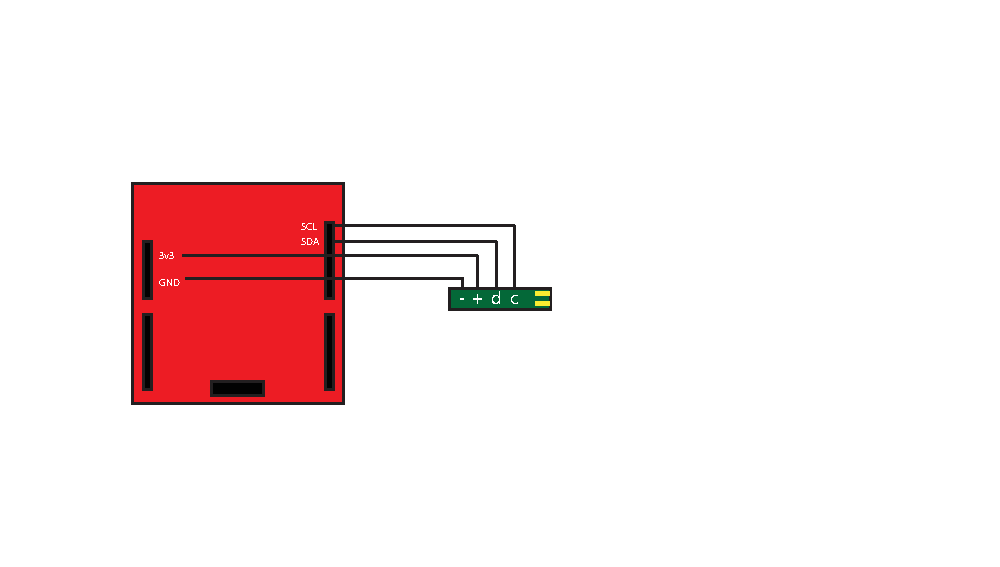
\includegraphics[scale=0.7]{Figures/NunchuckConnection}
  \end{center}
  \caption{Hardware connection of an nunchuk}
  \label{fig:nunchuk_connect}
\end{wrapfigure}




It is possible to use both the Gameduino 2 and Wii
nunchuk at the same time, even though they use same slots.
Gameduino 2 uses an ISP interface, while the Wii nunchuk uses an I2C interface.


\subsection*{I2C}
The I2C is a hardware wire interface, which is used by the Wii nunchuk adapter. This bus
interface allows easy communication between components and only requires two
bus lines. These lines are both bidirectional. These bus lines are called SCL
(Serial Clock Line) and SDA (Serial Data Line).
